% Options for packages loaded elsewhere
\PassOptionsToPackage{unicode}{hyperref}
\PassOptionsToPackage{hyphens}{url}
%
\documentclass[
  french,
]{article}
\usepackage{amsmath,amssymb}
\usepackage{lmodern}
\usepackage{ifxetex,ifluatex}
\ifnum 0\ifxetex 1\fi\ifluatex 1\fi=0 % if pdftex
  \usepackage[T1]{fontenc}
  \usepackage[utf8]{inputenc}
  \usepackage{textcomp} % provide euro and other symbols
\else % if luatex or xetex
  \usepackage{unicode-math}
  \defaultfontfeatures{Scale=MatchLowercase}
  \defaultfontfeatures[\rmfamily]{Ligatures=TeX,Scale=1}
\fi
% Use upquote if available, for straight quotes in verbatim environments
\IfFileExists{upquote.sty}{\usepackage{upquote}}{}
\IfFileExists{microtype.sty}{% use microtype if available
  \usepackage[]{microtype}
  \UseMicrotypeSet[protrusion]{basicmath} % disable protrusion for tt fonts
}{}
\makeatletter
\@ifundefined{KOMAClassName}{% if non-KOMA class
  \IfFileExists{parskip.sty}{%
    \usepackage{parskip}
  }{% else
    \setlength{\parindent}{0pt}
    \setlength{\parskip}{6pt plus 2pt minus 1pt}}
}{% if KOMA class
  \KOMAoptions{parskip=half}}
\makeatother
\usepackage{xcolor}
\IfFileExists{xurl.sty}{\usepackage{xurl}}{} % add URL line breaks if available
\IfFileExists{bookmark.sty}{\usepackage{bookmark}}{\usepackage{hyperref}}
\hypersetup{
  pdftitle={Un éditeur orienté ligne},
  pdfauthor={Julien Blanchon},
  pdflang={fr-FR},
  pdfkeywords={tob, java, midi, piano},
  hidelinks,
  pdfcreator={LaTeX via pandoc}}
\urlstyle{same} % disable monospaced font for URLs
\usepackage{listings}
\newcommand{\passthrough}[1]{#1}
\lstset{defaultdialect=[5.3]Lua}
\lstset{defaultdialect=[x86masm]Assembler}
\usepackage{graphicx}
\makeatletter
\def\maxwidth{\ifdim\Gin@nat@width>\linewidth\linewidth\else\Gin@nat@width\fi}
\def\maxheight{\ifdim\Gin@nat@height>\textheight\textheight\else\Gin@nat@height\fi}
\makeatother
% Scale images if necessary, so that they will not overflow the page
% margins by default, and it is still possible to overwrite the defaults
% using explicit options in \includegraphics[width, height, ...]{}
\setkeys{Gin}{width=\maxwidth,height=\maxheight,keepaspectratio}
% Set default figure placement to htbp
\makeatletter
\def\fps@figure{htbp}
\makeatother
\setlength{\emergencystretch}{3em} % prevent overfull lines
\providecommand{\tightlist}{%
  \setlength{\itemsep}{0pt}\setlength{\parskip}{0pt}}
\setcounter{secnumdepth}{-\maxdimen} % remove section numbering
\ifxetex
  % Load polyglossia as late as possible: uses bidi with RTL langages (e.g. Hebrew, Arabic)
  \usepackage{polyglossia}
  \setmainlanguage[]{french}
\else
  \usepackage[main=french]{babel}
% get rid of language-specific shorthands (see #6817):
\let\LanguageShortHands\languageshorthands
\def\languageshorthands#1{}
\fi
\ifluatex
  \usepackage{selnolig}  % disable illegal ligatures
\fi

\title{Un éditeur orienté ligne}
\usepackage{etoolbox}
\makeatletter
\providecommand{\subtitle}[1]{% add subtitle to \maketitle
  \apptocmd{\@title}{\par {\large #1 \par}}{}{}
}
\makeatother
\subtitle{TP 10}
\author{\href{mailto:julien.blanchon@etu.toulouse-inp.fr}{Julien
Blanchon}}
\date{1 Mars 2020}

\begin{document}
\maketitle

\renewcommand*\contentsname{Table des matières}
{
\setcounter{tocdepth}{3}
\tableofcontents
}
\hypertarget{exercice-1-comprendre-larchitecture-de-luxe9diteur-orientuxe9-ligne}{%
\section{Exercice 1 : Comprendre l'architecture de l'éditeur orienté
ligne}\label{exercice-1-comprendre-larchitecture-de-luxe9diteur-orientuxe9-ligne}}

L'application « éditeur orienté ligne » a été commencée. Il vous est
demandé de la compléter.

\hypertarget{exuxe9cuter-lapplication}{%
\subsection{1.1 Exécuter l'application}\label{exuxe9cuter-lapplication}}

\emph{Exécuter l'application.} Constater que le menu textuel est
opérationnel.

Le menu textuel est bien opérationnel.

\hypertarget{comprendre-larchitecture}{%
\subsection{1.2. Comprendre
l'architecture}\label{comprendre-larchitecture}}

\emph{Comprendre l'architecture.} Vérifier que le code respecte le
diagramme de classe fourni.

\begin{figure}
\centering
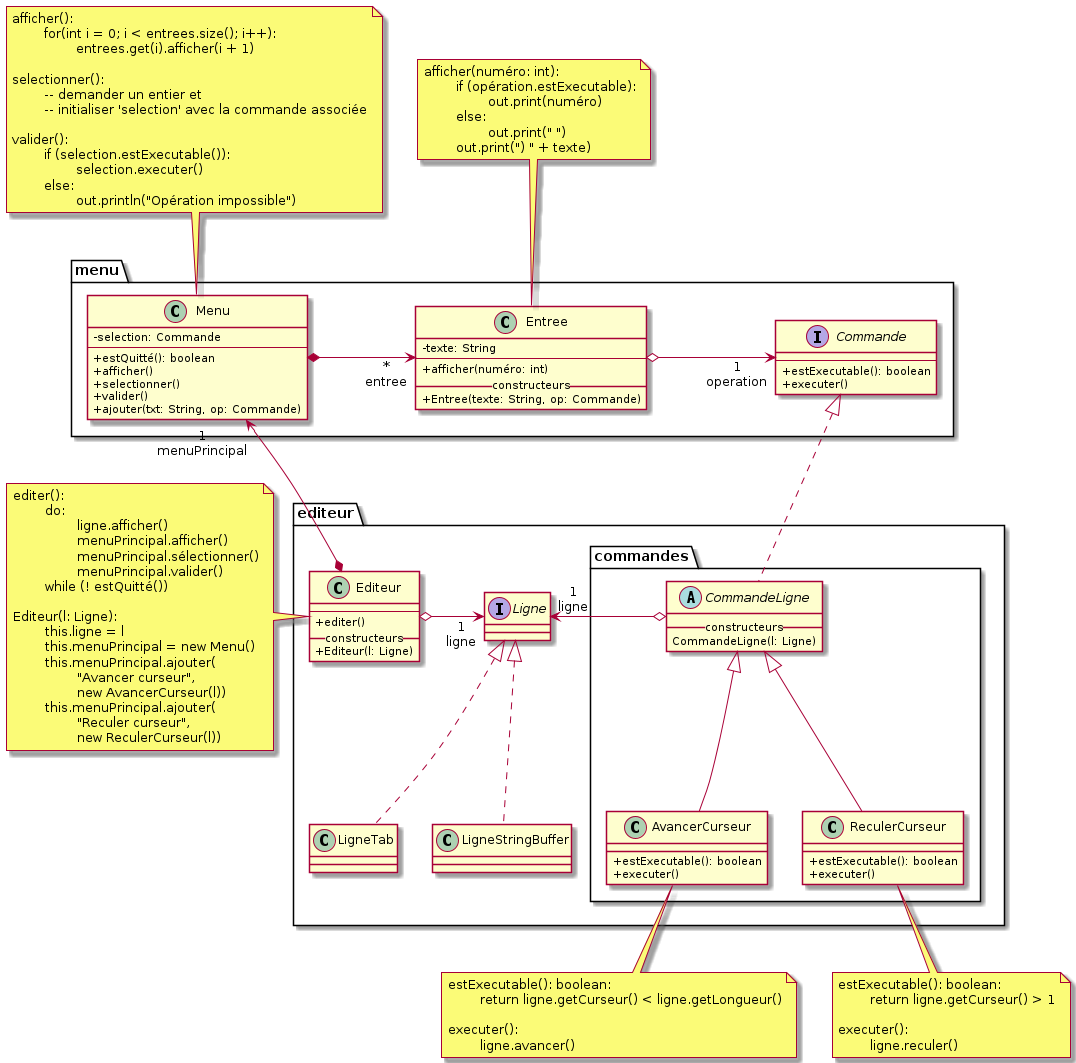
\includegraphics{editeur-menu.png}
\caption{Diagramme de classe de l'éditeur menu}
\end{figure}

OK !

\hypertarget{compluxe9ter-les-commandes.}{%
\subsection{1.3. Compléter les
commandes.}\label{compluxe9ter-les-commandes.}}

\emph{Compléter les commandes.} Ajouter deux nouvelles commandes au
menu. La première per- met de ramener le curseur sur le premier
caractère de la ligne (touche « 0 » en vi). La seconde permet de
supprimer le caractère sous le curseur (touche « x » en vi).

\begin{lstlisting}[language=Java]
# editeur/commande/CommandeSupprimerSousCurseur.java
\end{lstlisting}

\end{document}
